\documentclass[tikz,border=6pt]{standalone}
\usepackage{pgfplots}
\pgfplotsset{compat=1.18}
\usepgfplotslibrary{colormaps}
\usetikzlibrary{arrows, arrows.meta, calc}
\usetikzlibrary{decorations.markings}


\usepackage{amssymb,amsmath,mathtools}

\usepackage[T1]{fontenc}
\usepackage[utf8]{inputenc}
\usepackage{newpxtext,newpxmath}
\usepackage{sectsty}

\renewcommand{\Re}{\operatorname{\mathrm{Re}}}
\renewcommand{\Im}{\operatorname{\mathrm{Im}}}

\begin{document}
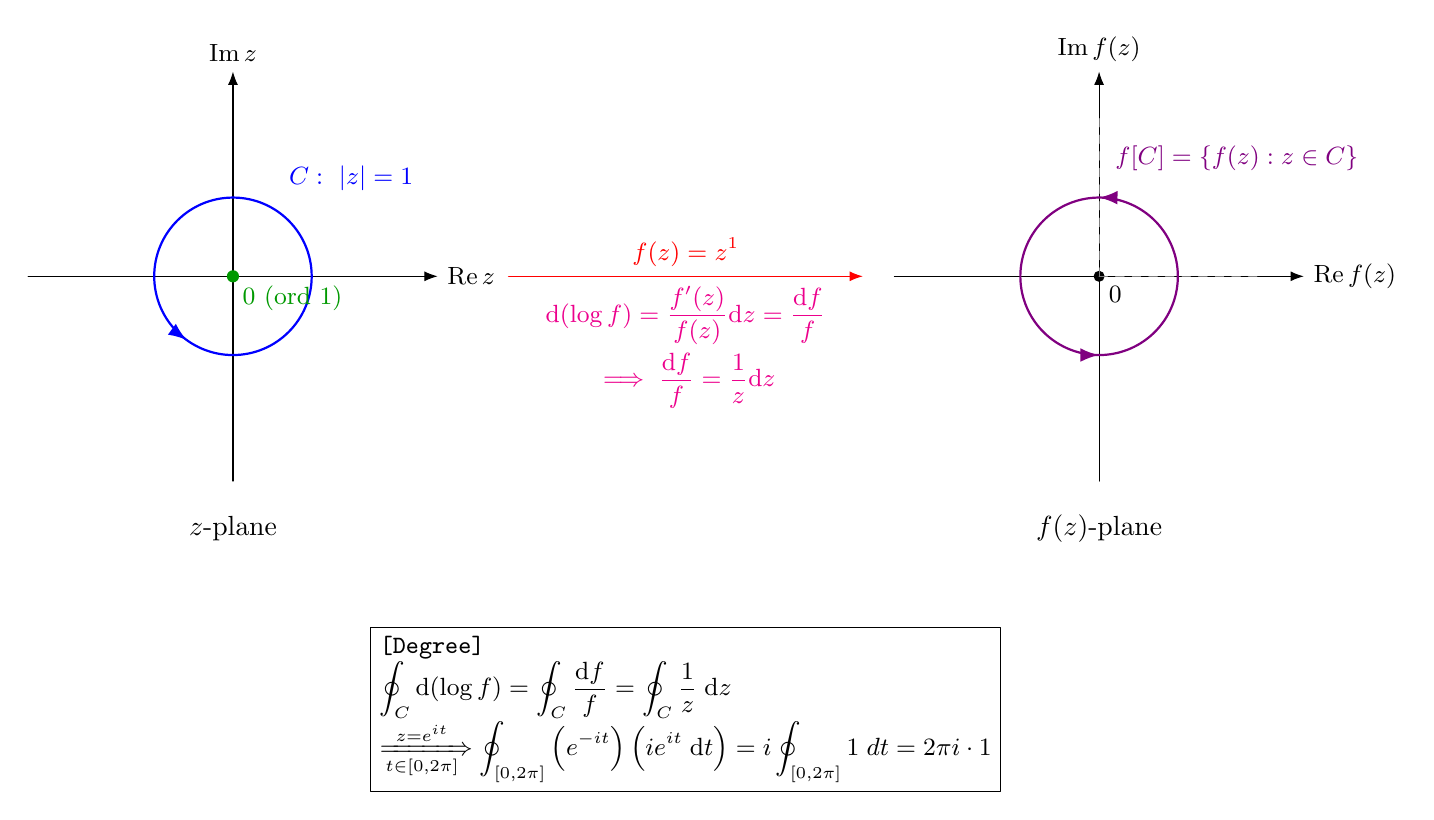
\begin{tikzpicture}[>=Latex, line cap=round, line join=round, font=\small]
%========================
% Left: z-plane
%========================
\begin{scope}[shift={(0,0)}]
	\node[font=\normalsize] at (0,-3.2) {$z$-plane};
	% axes
	\draw[->] (-2.6,0)--(2.6,0) node[right] {$\Re z$};
	\draw[->] (0,-2.6)--(0,2.6) node[above] {$\Im z$};
	% unit circle C (positively oriented)
	\draw[blue,thick,postaction={decorate},
	decoration={markings, mark=at position 0.65 with {\arrow{>}}}]
	(0,0) circle (1);
	\node[blue] at (1.5,1.25) {$C:\ |z|=1$};
	% zero at 0 (order 1)
	\fill[green!60!black] (0,0) circle(2.2pt) node[below right] {$0$ (ord $1$)};
%	\node[green!60!black] at (-1.7,1.7) {zeros: at $0$};
%	\node[red] at (-1.7,-1.7) {poles: none};
\end{scope}

% function label
\draw[->, red] (3.5,0) -- (8,0) node[midway, above, align=center] {$\displaystyle
	f(z)=z^1$};
\draw[->, magenta, opacity=0] (3.5,0) -- (8,0) node[midway, below, align=center, opacity=1] {
	$\displaystyle\mathrm{d}(\log f)=\frac{f'(z)}{f(z)}\mathrm{d}z=\frac{\mathrm{d}f}{f}$\\ [2pt]
	$\displaystyle\implies\frac{\mathrm{d}f}{f}=\frac{1}{z}\mathrm{d}z$};

\node[draw=black, align=left] at (5.75,-5.5) {
	\texttt{[Degree]}\\
	$\displaystyle
	\oint_C \mathrm{d}(\log f)=\oint_C \frac{\mathrm{d}f}{f}=\oint_C \frac{1}{z}\; \mathrm{d}z$ \\
	$\displaystyle\xRightarrow[{t\in[0,2\pi]}]{z=e^{it}}\oint_{[0,2\pi]}\left(e^{-it}\right)\left(ie^{it}\; \mathrm{d}t\right)=i\oint_{[0,2\pi]}1\; dt=2\pi i\cdot 1$
%	\\ [10pt]
%	\texttt{[Coefficient]}\\
%	$\displaystyle a_0=\frac{f(0)}{0!}=\frac{1}{2\pi i}\!\oint_C \frac{f(\zeta)}{\zeta}\,d\zeta=0$ \\
%	$\displaystyle a_1=\frac{f'(0)}{1!}=\frac{1}{2\pi i}\!\oint_C \frac{f(\zeta)}{\zeta^{2}}\,d\zeta=1$\\
%	$a_n= 0$ for $n\geq 2$
};

%========================
% Right: f(z)-plane
%========================
\begin{scope}[shift={(11,0)}]
	\node[font=\normalsize] at (0,-3.2) {$f(z)$-plane};
	% axes
	\draw[->] (-2.6,0)--(2.6,0) node[right] {$\Re f(z)$};
	\draw[->] (0,-2.6)--(0,2.6) node[above] {$\Im f(z)$};
	% origin
	\fill (0,0) circle(2pt) node[below right] {$0$};
	% image curve f(C) = C (identity map)
	\draw[violet,thick,
	postaction={decorate},
	decoration={markings,
		mark=at position 0.25 with {\arrow{>}},
		mark=at position 0.75 with {\arrow{>}}}]
	plot[domain=0:6.283, samples=400] ({1*cos(\x r)},{1*sin(\x r)});
	\node[violet] at (1.75,1.5) {$f[C]=\{f(z):z\in C\}$};
	\draw[gray,dashed] (0,0) -- (2.1,0);
	\draw[gray,dashed] (0,0) -- (0,2.1);
\end{scope}
\end{tikzpicture}
\end{document}